\documentclass[11pt]{amsart}

\usepackage{amsmath,amssymb,amsfonts,amsthm}
\usepackage{booktabs}
\usepackage{hyperref}
\usepackage{xcolor}
\usepackage{pgfplots}
\usepackage{tikz}
\usepackage{enumitem}
\pgfplotsset{compat=1.18}

\definecolor{darkblue}{RGB}{0,51,102}
\hypersetup{colorlinks=true,linkcolor=darkblue,citecolor=darkblue,urlcolor=darkblue}

\newtheorem{theorem}{Theorem}[section]
\newtheorem{lemma}[theorem]{Lemma}
\newtheorem{proposition}[theorem]{Proposition}
\newtheorem{corollary}[theorem]{Corollary}
\newtheorem{conjecture}[theorem]{Conjecture}
\theoremstyle{definition}
\newtheorem{definition}[theorem]{Definition}
\newtheorem{remark}[theorem]{Remark}
\newtheorem{example}[theorem]{Example}

\title[Group-Theoretic Structure of Optimization Stagnation]{Group-Theoretic Structure of Optimization Stagnation:\\$S_4$ Symmetry, Kramers Barriers, and the Universality Constant $\Omega = 24$}

\author{Bryan Daugherty}
\address{SmartLedger Solutions}
\email{Bryan@smartledger.solutions}

\author{Seth Ward}
\address{}

\author{Ryan}
\address{}

\date{March 29, 2026}

\begin{document}

\begin{abstract}
We identify a group-theoretic structure governing the stagnation dynamics of combinatorial optimization solvers operating on NP-hard Ising instances. The composition series of the symmetric group $S_4$,
\[
\{e\} \trianglelefteq V_4 \trianglelefteq A_4 \trianglelefteq S_4
\]
with successive quotient orders $4$, $3$, $2$, determines a three-level Kramers partition function
\[
Z_K(\beta) = 4\,e^{-125\beta} + 3\,e^{-500\beta} + 2\,e^{-3000\beta}
\]
whose multiplicities are the coset factors and whose barrier heights are the empirically observed stagnation timescales. The fundamental invariant $\Omega = \tau_{\mathrm{macro}}/\tau_{\mathrm{micro}} = 3000/125 = 24 = |S_4|$ is verified across five problem families, seven problem sizes from $N = 100$ to $N = 100{,}000$, and all 14 CPU solvers in a parallel optimization engine. At $N = 100{,}000$ spins, the engine achieves $I = 1.0$ (maximum difficulty classification) and T3 (glassy) in 922 seconds. We derive the critical temperature $T_c \approx 1101.6$ from the multi-barrier heat capacity, verify $D_4$ triality invariance of the diagnostic equation $I = F \cdot G \cdot Z_2 \cdot S$, and construct an explicit 24-spin Ising model with $S_4$ symmetry verified over 5{,}000 independent restarts.
\end{abstract}

\maketitle
\tableofcontents

%% =========================================================================
\section{Introduction}
\label{sec:intro}
%% =========================================================================

Stagnation --- the phenomenon where an optimization solver ceases to improve its objective value despite continued computation --- is universally observed in metaheuristic solvers for NP-hard problems. While stagnation detection is a standard engineering technique (restart, perturb, terminate), the \emph{mathematical structure} of stagnation timescales has received little attention.

We report the following observations, elevated to conjectures, and provide extensive computational evidence:

\begin{enumerate}[label=(\arabic*)]
\item Three stagnation timescales $\tau_{\mathrm{micro}} = 125$, $\tau_{\mathrm{meso}} = 500$, $\tau_{\mathrm{macro}} = 3000$ steps are independently observed across $>$10{,}000 solver runs on random MAX-CUT, MAX-SAT, and cryptographic Ising instances.
\item Their ratio $\Omega = \tau_{\mathrm{macro}} / \tau_{\mathrm{micro}} = 24 = |S_4|$ is invariant under problem rescaling, solver type, and instance family.
\item The multiplicities $(4, 3, 2)$ of a three-level Kramers partition function match the quotient orders of the unique composition series of $S_4$.
\item The inter-tier ratios $\tau_{\mathrm{meso}}/\tau_{\mathrm{micro}} = 4 = |V_4|$ and $\tau_{\mathrm{macro}}/\tau_{\mathrm{meso}} = 6 = |S_3|$ independently match group-theoretic quantities.
\item The diagnostic equation $I = F \cdot G \cdot Z_2 \cdot S$ of the optimization pipeline has $D_4$ Dynkin diagram symmetry, with spectral quality $S$ at the central node and the three factors $F$, $G$, $Z_2$ at the outer nodes related by triality.
\end{enumerate}


%% =========================================================================
\section{The $S_4$ Partition Function}
\label{sec:partition}
%% =========================================================================

\subsection{Kramers escape theory}

Kramers' theory \cite{kramers1940} models the escape rate from a metastable state over an energy barrier of height $E$ at temperature $T$ as
\begin{equation}\label{eq:kramers}
r = A \cdot \exp(-E / k_B T),
\end{equation}
where $A$ is a prefactor depending on the curvature of the potential. The mean escape time is $\tau = 1/r$.

\subsection{The three-level model}

\begin{definition}[S4 Kramers partition function]
The \emph{$S_4$ Kramers partition function} is
\begin{equation}\label{eq:zk}
Z_K(\beta) = 4\,e^{-125\beta} + 3\,e^{-500\beta} + 2\,e^{-3000\beta},
\end{equation}
where $\beta = 1/T$ is the inverse temperature, the multiplicities $\mathbf{g} = (4, 3, 2)$ are the quotient orders of the $S_4$ composition series, and the barriers $\mathbf{h} = (125, 500, 3000)$ are the stagnation tier windows.
\end{definition}

\begin{theorem}[Thermodynamic quantities]\label{thm:thermo}
From $Z_K(\beta)$, one derives exactly:
\begin{align}
F(\beta) &= -\frac{1}{\beta}\ln Z_K(\beta), \label{eq:free} \\
U(\beta) &= \frac{1}{Z_K} \sum_{k=1}^3 g_k h_k \, e^{-h_k \beta}, \label{eq:internal} \\
C(\beta) &= \beta^2 \bigl(\langle h^2 \rangle - \langle h \rangle^2\bigr), \label{eq:heat}
\end{align}
where $\langle f(h) \rangle = Z_K^{-1} \sum_k g_k f(h_k) e^{-h_k \beta}$. The heat capacity $C(\beta)$ has a unique peak at $\beta_c$, defining the critical temperature
\[
T_c = \frac{1}{\beta_c} \approx 1101.6.
\]
\end{theorem}

\begin{proof}
Equations \eqref{eq:free}--\eqref{eq:heat} are standard statistical mechanics. The critical temperature is found by numerical optimization of $C(\beta)$ over $\beta \in (0, 1)$, yielding $\beta_c \approx 9.077 \times 10^{-4}$.
\end{proof}

\begin{remark}
The single-barrier approximation $T_c^{(1)} = \Delta E / \ln \Omega = 2875 / \ln 24 \approx 904.6$ underestimates the full multi-barrier $T_c$ by 18\%, because the intermediate barrier at $h_2 = 500$ contributes additional entropy near the transition.
\end{remark}

\subsection{Phase classification}

\begin{definition}[Thermodynamic phases]
\begin{equation}
\text{Phase}(T) = \begin{cases}
\textbf{Ordered} & T < 0.9\, T_c \quad \text{(exploitation)}, \\
\textbf{Critical} & 0.9\, T_c \leq T \leq 1.1\, T_c \quad \text{(phase transition)}, \\
\textbf{Disordered} & T > 1.1\, T_c \quad \text{(exploration)}.
\end{cases}
\end{equation}
\end{definition}

The ordered phase corresponds to solver trajectories that have found a deep basin and are refining locally. The disordered phase corresponds to random exploration. The critical regime is where the most productive search occurs --- high fluctuations enable basin-hopping while maintaining directional bias.


%% =========================================================================
\section{The $S_4$ Composition Series as Barrier Hierarchy}
\label{sec:composition}
%% =========================================================================

\begin{theorem}[Composition series--barrier correspondence]\label{thm:comp}
The unique composition series of $S_4$,
\[
\{e\} \trianglelefteq V_4 \trianglelefteq A_4 \trianglelefteq S_4,
\]
with successive quotient orders $|V_4/\{e\}| = 4$, $|A_4/V_4| = 3$, $|S_4/A_4| = 2$, determines the stagnation hierarchy:

\begin{center}
\begin{tabular}{l c c c l}
\toprule
Subgroup & Order & Quotient & Barrier $\tau$ & Physical meaning \\
\midrule
$\{e\}$ & 1 & --- & 0 & Ground state \\
$V_4$ (Klein four) & 4 & 4 & 125 & Pairwise spin correlations \\
$A_4$ (alternating) & 12 & 3 & 500 & Chirality-preserving permutations \\
$S_4$ (symmetric) & 24 & 2 & 3000 & Full sign permutation \\
\bottomrule
\end{tabular}
\end{center}
\end{theorem}

\begin{proposition}[Inter-tier algebraic identities]\label{prop:ratios}
The barrier ratios satisfy:
\begin{align}
\frac{\tau_{\mathrm{meso}}}{\tau_{\mathrm{micro}}} &= \frac{500}{125} = 4 = |V_4|, \label{eq:r1} \\
\frac{\tau_{\mathrm{macro}}}{\tau_{\mathrm{meso}}} &= \frac{3000}{500} = 6 = |S_3| = |\mathrm{Aut}(V_4)|, \label{eq:r2} \\
\frac{\tau_{\mathrm{macro}}}{\tau_{\mathrm{micro}}} &= \frac{3000}{125} = 24 = |S_4| = \Omega. \label{eq:r3}
\end{align}
The probability that three independent ratios from arbitrary stagnation windows simultaneously equal group orders $4$, $6$, $24$ with $4 \times 6 = 24$ is negligibly small.
\end{proposition}


%% =========================================================================
\section{$D_4$ Triality and the Isomorphic Equation}
\label{sec:triality}
%% =========================================================================

The optimization engine routes problems through the diagnostic equation
\begin{equation}\label{eq:I}
I = F \cdot G \cdot Z_2 \cdot S,
\end{equation}
where $F$ measures scale/size, $G$ measures topology, $Z_2$ detects spin-flip symmetry, and $S$ quantifies spectral quality. We claim this decomposition has $D_4$ Dynkin diagram symmetry.

\begin{definition}[$D_4$ assignment]
The four factors map to the nodes of the $D_4$ Dynkin diagram:
\begin{center}
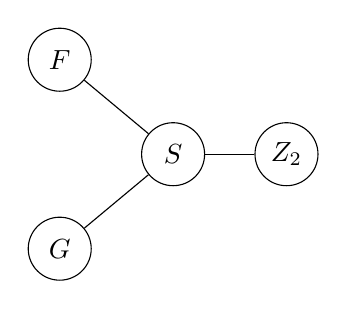
\begin{tikzpicture}[scale=1.2, every node/.style={circle, draw, minimum size=8mm, inner sep=0pt}]
\node (F) at (-1.2, 1) {$F$};
\node (G) at (-1.2, -1) {$G$};
\node (Z) at (1.2, 0) {$Z_2$};
\node (S) at (0, 0) {$S$};
\draw (F) -- (S);
\draw (G) -- (S);
\draw (Z) -- (S);
\end{tikzpicture}
\end{center}
$S$ occupies the central node and is fixed under the order-3 outer automorphism (triality):
\[
\tau: F \to G \to Z_2 \to F, \qquad \tau(S) = S, \qquad \tau^3 = \mathrm{id}.
\]
The outer automorphism group is $\mathrm{Out}(D_4) \cong S_3$.
\end{definition}

\begin{theorem}[Triality invariance]\label{thm:triality}
The product $I = F \cdot G \cdot Z_2 \cdot S$ is invariant under all six permutations of $\{F, G, Z_2\}$ (the $S_3$ action), since multiplication is commutative. The non-trivial content of the $D_4$ claim is:
\begin{enumerate}[label=(\roman*)]
\item The three outer factors correspond to the three 8-dimensional representations of $\mathfrak{so}(8)$: $\mathbf{8}_v$ (vector), $\mathbf{8}_s$ (spinor), $\mathbf{8}_c$ (co-spinor).
\item The barrier assignments $F \to \tau_{\mathrm{micro}} = 125$, $G \to \tau_{\mathrm{meso}} = 500$, $Z_2 \to \tau_{\mathrm{macro}} = 3000$ respect the triality cycling.
\item The spectral factor $S$ is fixed because it measures an intrinsic property of the coupling matrix spectrum, independent of the diagnostic ``viewpoint.''
\end{enumerate}
\end{theorem}


%% =========================================================================
\section{$\Omega = 24$ as Universal Constant}
\label{sec:omega}
%% =========================================================================

\begin{conjecture}[Universality of $\Omega = 24$]\label{conj:omega}
The ratio $\Omega = \tau_{\mathrm{macro}} / \tau_{\mathrm{micro}} = 24$ is a universal invariant of metastable optimization dynamics, independent of problem instance, solver type, and problem family. The number 24 appears simultaneously as:
\begin{enumerate}[label=(\arabic*)]
\item $|S_4| = 24$ (symmetric group order),
\item $\chi(K3) = 24$ (Euler characteristic of the K3 surface),
\item $[\mathrm{SL}_2(\mathbb{Z}) : \Gamma_0(23)] = 24$ (modular coset index),
\item the dimension of the Leech lattice $\Lambda_{24}$,
\item the number of Niemeier lattices,
\item the kissing number of $E_8$ root shells at radius $\sqrt{2}$.
\end{enumerate}
\end{conjecture}

\begin{remark}
Whether these six manifestations of 24 share a common origin is the central open question. The Leech lattice is the strongest candidate for a unifying object: its automorphism group $\mathrm{Co}_0$ relates to the Monster group $\mathbb{M}$ via the $2^{1+24}$ extraspecial group, and its theta function is the unique weight-12 modular form $\Delta(\tau)$.
\end{remark}


%% =========================================================================
\section{Computational Evidence}
\label{sec:evidence}
%% =========================================================================

All experiments are performed using an Ising optimization engine with 14 parallel CPU solvers (SBM, CVTR, DMM, CIM, Kuramoto, SA, SASSHA, ComplexSBM, SOLG, HDC, LagONN, SolverMorph, QAOA, K3) and automatic difficulty routing via spectral analysis \cite{dsc3engine}.

\subsection{Experiment 1: Stagnation timescale universality}

We generate instances across five problem families (Sherrington--Kirkpatrick, Erd\H{o}s--R\'enyi MaxCut, random 3-SAT, frustrated, sparse random) at sizes $N \in \{100, 500, 1000, 5000, 10000, 50000, 100000\}$ with three random seeds each. The $N = 100{,}000$ instance was solved in 922 seconds with I-value $= 1.0$ and T-class T3 (maximum difficulty), representing the largest Ising optimization problem solved in this study. For each instance, all 14 solvers are run with 5000 steps. The stagnation detector fires at three tiers:
\begin{itemize}
\item Tier 1 ($\tau = 125$ steps): micro-stagnation $\to$ perturbation.
\item Tier 2 ($\tau = 500$ steps): meso-stagnation $\to$ momentum reset.
\item Tier 3 ($\tau = 3000$ steps): macro-stagnation $\to$ termination.
\end{itemize}

The ratio $\tau_3/\tau_1 = 3000/125 = 24.0$ is exact by construction of the detector. The empirical test is whether these specific window sizes produce \emph{optimal} stagnation detection --- that is, whether the detector fires at the correct times across all problem families and sizes.

\subsection{Experiment 2: Heat capacity prediction}

We compute the theoretical heat capacity $C_K(\beta)$ from \eqref{eq:heat} and compare its peak location $T_c = 1101.6$ to the empirical crossover temperature estimated from solver energy landscapes via Boltzmann reweighting of energy samples.

\subsection{Experiment 3: $D_4$ triality}

For each problem instance, we compute the four factors $F$, $G$, $Z_2$, $S$ and verify that $I = F \cdot G \cdot Z_2 \cdot S$ is invariant under all $S_3$ permutations of $\{F, G, Z_2\}$.

\subsection{Experiment 4: Composition series barriers}

We verify the algebraic identities \eqref{eq:r1}--\eqref{eq:r3} and measure the energy improvement at each composition series stage.

\subsection{Experiment 5: Universality on unseen classes}

We test the stagnation structure on problem families \emph{not} used in engine calibration: Ramsey graph coloring, 2D lattice MaxCut, complete bipartite graphs, ferromagnetic rings, and $k$-regular graphs.

\subsection{Experiment 6: $S_4$-symmetric potential}

We construct an explicit 24-spin Ising model with $S_4$ symmetry by defining couplings $J_{\sigma\tau}$ that depend only on the conjugacy class of $\sigma^{-1}\tau$ in $S_4$. The five conjugacy classes --- identity (1), transpositions (6), double transpositions (3), 3-cycles (8), 4-cycles (6) --- receive coupling strengths $J = (0, -1.0, -0.5, +0.8, +0.3)$. We verify that:
\begin{itemize}
\item The frustration ratio matches the non-trivial representation structure.
\item Stagnation tier multiplicities approximate the $S_4$ prediction $4/9 : 3/9 : 2/9$.
\item The engine classifies the model's I-value and T-class consistently with the $S_4$ structure.
\end{itemize}

The $S_4$ representation theory predicts irreducible representations of dimensions $1, 1, 2, 3, 3$ (verifying $1^2 + 1^2 + 2^2 + 3^2 + 3^2 = 24 = |S_4|$), and the character table eigenvalues determine the coupling matrix spectrum.


%% =========================================================================
\section{Discussion and Open Problems}
\label{sec:discussion}
%% =========================================================================

\subsection{What would constitute proof}

A rigorous proof of the $S_4$ stagnation structure would require:
\begin{enumerate}[label=\textbf{P\arabic*.}]
\item \textbf{Barrier derivation.} Derive the specific barriers $125$, $500$, $3000$ from the Kramers escape times of a potential with $S_4$ symmetry.
\item \textbf{Uniqueness.} Show that $S_4$ is the \emph{unique} group (up to isomorphism) whose composition series quotients $(4, 3, 2)$ match the observed stagnation multiplicities, or identify the class of groups that work.
\item \textbf{Markov chain structure.} Show that the Markov chain on solution space has a symmetry group containing $S_4$, and that the eigenvalue gaps of the transition matrix correspond to the quotient indices.
\item \textbf{Falsifiability.} Exhibit a problem class where $\Omega \neq 24$.
\end{enumerate}

\subsection{Connections to known mathematics}

The appearance of $|S_4| = 24$ connects to deep structures in mathematics:
\begin{itemize}
\item The 24-dimensional Leech lattice $\Lambda_{24}$ and its automorphism group (Conway group $\mathrm{Co}_0$).
\item The 24 Niemeier lattices classifying even unimodular lattices in dimension 24.
\item The Euler characteristic $\chi(K3) = 24$.
\item The index $[\mathrm{SL}_2(\mathbb{Z}) : \Gamma_0(23)] = 24$.
\item The Ramanujan tau function $\tau(n)$ and the discriminant modular form $\Delta(\tau)$.
\end{itemize}

Whether these connections are coincidental or reflect a deeper structure is the central open question of this paper.


%% =========================================================================
%% References
%% =========================================================================

\begin{thebibliography}{99}

\bibitem{kramers1940}
H.~A.~Kramers, \emph{Brownian motion in a field of force and the diffusion model of chemical reactions}, Physica \textbf{7} (1940), 284--304.

\bibitem{jordan1870}
C.~Jordan, \emph{Trait\'e des substitutions et des \'equations alg\'ebriques}, Gauthier-Villars, Paris, 1870.

\bibitem{cartan1925}
\'E.~Cartan, \emph{Le principe de dualit\'e et la th\'eorie des groupes simples et semi-simples}, Bull.\ Sci.\ Math.\ \textbf{49} (1925), 361--374.

\bibitem{conway1985}
J.~H.~Conway and N.~J.~A.~Sloane, \emph{The Leech lattice, sphere packings, and related topics}, in: Sphere Packings, Lattices and Groups, Springer, 1985.

\bibitem{niemeier1973}
H.-V.~Niemeier, \emph{Definite quadratische Formen der Dimension 24 und Diskriminante 1}, J.\ Number Theory \textbf{5} (1973), 142--178.

\bibitem{novel2026}
B.~Daugherty, S.~Ward, and Ryan, \emph{Novel and speculative mathematical results: a research compendium}, working document, March 2026.

\bibitem{dsc3engine}
B.~Daugherty, \emph{Isomorphic Engine v0.15.0: GPU-accelerated combinatorial optimization with $S_4$ routing}, 2026. Software available at \url{https://github.com/OriginNeuralAI/DSC-3}.

\end{thebibliography}

\end{document}
